%! suppress = FileNotFound
\documentclass[conference]{IEEEtran}
\IEEEoverridecommandlockouts


\usepackage{cite}
\usepackage{csquotes}
\usepackage{graphicx}
\usepackage{textcomp}
\usepackage{xcolor}

%! suppress = DiscouragedUseOfDef
\def\BibTeX{{%! suppress = PrimitiveStyle
\rm B\kern-.05em{%! suppress = PrimitiveStyle
\sc i\kern-.025em b}\kern-.08em
T\kern-.1667em\lower.7ex\hbox{E}\kern-.125emX}}

\begin{document}
\title{'Some title'}

\author{
	\IEEEauthorblockN{1
		\textsuperscript{st} Bachmann Lucius
	}
	\IEEEauthorblockA{
		\textit{Department of Informatics} \\
		\textit{University of Zurich}\\
		Zurich, Switzerland \\
		lucius.bachmann@gmx.ch
	}
}

\maketitle

\begin{abstract}
	Cloud computing is pervasive in the software industry.
With the advancement of web technology it is now possible to fulfill most of the computing needs as a service
in the cloud.
The services offering cloud services are also using other cloud services to perform their computing.
The development effort to develop and deploy an application to the cloud becomes less every year.
This also allows to use testing tools in the cloud to speed up the development and reduce cost for the development.
The following paragraphs will show how small to medium sized applications can leverage the cloud to test their application.

\end{abstract}

\begin{IEEEkeywords}
	component, formatting, style, styling, insert
\end{IEEEkeywords}

\section{Introduction}

\subsection{Technological terms}

\subsubsection{OCI containers and docker}

\subsubsection{Kubernetes}

\subsubsection{Helm}

\subsubsection{Github Actions}

\section{eCamp Version 3}

eCamp is a web application to help with organising camps for youth organisations like the
scouts, YMCA (Young Men Christian Organisation)\cite{ymca-website} and YWCA or the Jubla.
It allows to collaboratively schedule the activities during the camp and to plan them in detail
according to the regulations of the swiss federal support program for sport activities (Y+S) with young people\cite{J+S-Website,ecamp3-website}.
eCamp version 2 is live since at least 2010\cite{ecamp2-first-commit} and was already used to plan a lot of camps.
The new version 3 is in development since 5 years\cite{ecamp3-website} with the goal to separate frontend and backend and
to leverage known, active and newer frameworks for frontend and backend for their bug and security fixes and
their new features to improve the usability, accessibility and maintainability of the application.

\subsubsection{Technology stack}

\subsubsection{Architecture}

The application uses 5 components depicted in figure\ref{fig:ecamp3-architecture}.
The frontend is a Vue application bundled with vite and served by a nginx web server.
The api is a PHP application using the API Platform framework which also served by a web server.
The print service is a nuxt application which lets the browserless container visit itself to render a printable
html of an activity, schedule or a whole camp and convert it to a pdf, which is then served back to the frontend.

\begin{figure}[h!]
	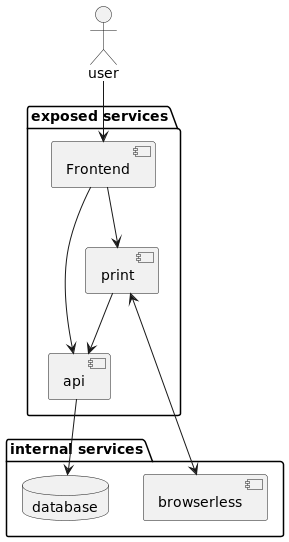
\includegraphics[height=\columnwidth]{sections/assets/ecamp3-architecture}
	\caption{eCamp V3 Architecture}
	\label{fig:ecamp3-architecture}
\end{figure}

\subsubsection{Deployment}

\section{Related work}

\section{Background}

\section{Method}

\section{Experiment}

\section{Conclusion}

\bibliographystyle{IEEEtran}
\bibliography{main}

\date{\today}



\newpage
%
\end{document}